\chapter{The impact of host interspecies diversity on the root associated microbiome and potential implications in agriculture.}

Joseph Edwards\footnote[1]{Department of Plant Biology, University of California, Davis}, John Kilmer\footnote[2]{College of Agriculture and Technology, Arkansas State University}, Christian Santos$^1$, Bao Nguyen$^1$, Gregory Phillips$^2$, and Venkatesan Sundaresan$^1$

\section{Abstract}

Plant roots assemble a distinct root-associated microbiota from the soil which can contribute beneficial properties to plant growth and performance. Previous studies have indicated that root-associated microbiomes are mainly constrained by environmental factors that act upon the broader soil microbial communities and that various root compartments pose as different niches for microbial colonization with the rhizosphere soil hosting the highest diversity of microbes and the root endosphere hosting the least. It was consistently found across various plant microbiome studies that genetic diversity within a host plant species contributes a minimal proportion of variance to root-associated microbiome differences. Thus, we were interested in quantifying the effect of host species specificity on root-associated microbiomes and whether this effect outweighs within host species microbiome diversity. We compiled published datasets from various plant microbiome studies and found that the environment that various host species are growing in is the largest determinant of root-associated microbiome structure and that rice has a relatively unique microbiome, presumably because it is cultivated under flooded (i.e. anaerobic conditions). To better understand how root-associated microbiomes vary across host plant species within a single environment, we sampled the roots of native plant species from a rice field along with roots from rice plants. We found host specificity to be a large factor contributing to microbiome variation and that rice plants host a larger proportion of methanogenic archaea than native plants growing in the same environment. The rhizosphere soil microbiome of rice was significantly more similar to unplanted soil microbial communities than were the rhizosphere microbiomes of native plants. By comparing rice plants grown in rice field soil vs rice plants grown in soil which has never cultivated rice, we established that this observation was at least in part due to continuous rice cultivation establishing a microbiome more similar to the rice rhizosphere. Together, these results indicate that different host plants acquire largely dissimilar root-associated microbiomes and that when rice is grown in dense monoculture, it shifts the overall soil microbiome to be more resemblant of the rice rhizosphere microbiome.

\section{Introduction}
Land plants growing in soil interact with a vast array of microbial diversity via their roots. Individual soil microbes have been shown to provide plants with beneficial effects including general growth promotion, pathogen exclusion, and protection against abiotic stresses \cite{Berendsen2012}. Plant-associated microbes, however, do not act in isolation and are part of a broader interconnected community, collectively known as the rhizosphere or root-associated microbiome \cite{Bulgarelli2013}. Harnessing the beneficial properties of the root-associated microbiome is of agricultural and biotechnological interest, yet the parameters governing their assembly are not fully understood \cite{Bulgarelli2013}. 

Plant roots host microbiomes that are distinct from the surrounding soil. Furthermore, root-associated microbiomes differ in composition between the rhizosphere soil and the root endosphere, with the latter having a significantly reduced microbial diversity than the former \cite{Lundberg2012,Bulgarelli2012,Edwards2015,Peiffer2013,Wagner2016,Zarraonaindia2015}. Genotypic diversity within a host plant species has a significant role in shaping the root-associated microbiome \cite{Lundberg2012,Wagner2016,Peiffer2013,Edwards2015}. It was recently reported that root-endosphere enriched microbiomes of Arabidopsis relatives are compositionally distinct in only a few taxonomic members, and the patterns of these differences are contradictory to host species phylogeny \cite{Schlaeppi2014}. Consistent with other studies, the microbiome variance partitioned to plant genotype was largely overshadowed by the variance partitioned to environmental factors (i.e. soil type, batch, field location and treatments), suggesting that plants from different, but related, species assemble a largely taxonomically conserved microbiome derived from a subset of the soil microbiome reservoir, which is affected by various environmental factors.

Asian rice (\textit{Oryza sativa}) is primarily cultivated under flooded conditions, a growth habit unique for cereal crop plants. We have previously characterized the rice root-associated microbiome, finding that root-associated microbiomes can be separated into 3 spatially and compositionally distinct compartments: the rhizosphere soil, the rhizoplane, and the endosphere. Rice genotype, despite including another cultivated rice species in this study (\textit{Oryza glaberrima}), was a very small explanatory variable for root-associated microbiome differences. These results suggest that interspecies variation between domesticated members of the \textit{Oryza} genus minimally affects the root-associated microbiome; however, it is unknown how root-associated microbiomes vary outside of the \textit{Oryza} genus when grown under the same flooded conditions. In this study, we sought to characterize the rice root-associated microbiome compared to other plant species.

\section{Results}
\subsection{Plant root-associated microbiomes are influenced by environmental conditions.}
To examine interspecies variation among root-associated microbiomes, we compiled plant rhizosphere microbiome sequencing data from 5 published datasets (Table 3.1). Primer choice during 16S rRNA gene sequencing experiments can cause significant variation in detectability of different taxa \cite{Debelius2016}, therefore we selected studies that sequenced the V4 region of the 16S rRNA gene. The sequences were clustered into operational taxonomic units (OTUs) based upon 97\% sequencing identity using the NINJA-OPS pipeline \cite{Al-Ghalith2016}. 

\begin{table}[ht]
\centering
\small
\definecolor{Gray}{gray}{0.9}
\caption[Table 3.1]{Plant hosts included in the meta-analysis study.}
\begin{tabular}{c|ccc}
\hline
\textbf{Organism}& \textbf{Common Name} & \textbf{Study} & \textbf{Sequencing Technology} \\
\hline
\rowcolor{Gray}
\textit{Oryza sativa}& Asian Rice & Edwards et al. \cite{Edwards2015} & Illumina \\
\textit{Zea mays}& Maize & Peiffer et al. \cite{Peiffer2013} & 454 \\
\rowcolor{Gray}
\textit{Boechera stricta}& Drummond's Rockcress & Wagner et al. \cite{Wagner2016} & Illumina \\
\textit{Cannabis spp.}& Cannabis & Winston et al. \cite{Winston2014} & 454 \\
\rowcolor{Gray}
\textit{Vitis vinifera}& Grape vine & Zarraonaindia et al. \cite{Zarraonaindia2015} & Illumina \\
\hline
\end{tabular}
\end{table}

We first examined how alpha diversity varies between the host species in each study (Fig. 3.1A). We found that alpha diversity significantly varied by host species and compartment (P < 2e-16 and P < 2e-16, respectively); however, this effect is confounded by sequencing depth (P < 2e-16). For example, the studies using 454 sequencing rather than Illumina sequencing had overall lower alpha diversity measurements and sequencing depth within samples, thus it was impossible to attribute significant differences in alpha diversity between the various studies to interspecies variation rather than technical or environmental variation. 

\begin{figure}[h]
\centering
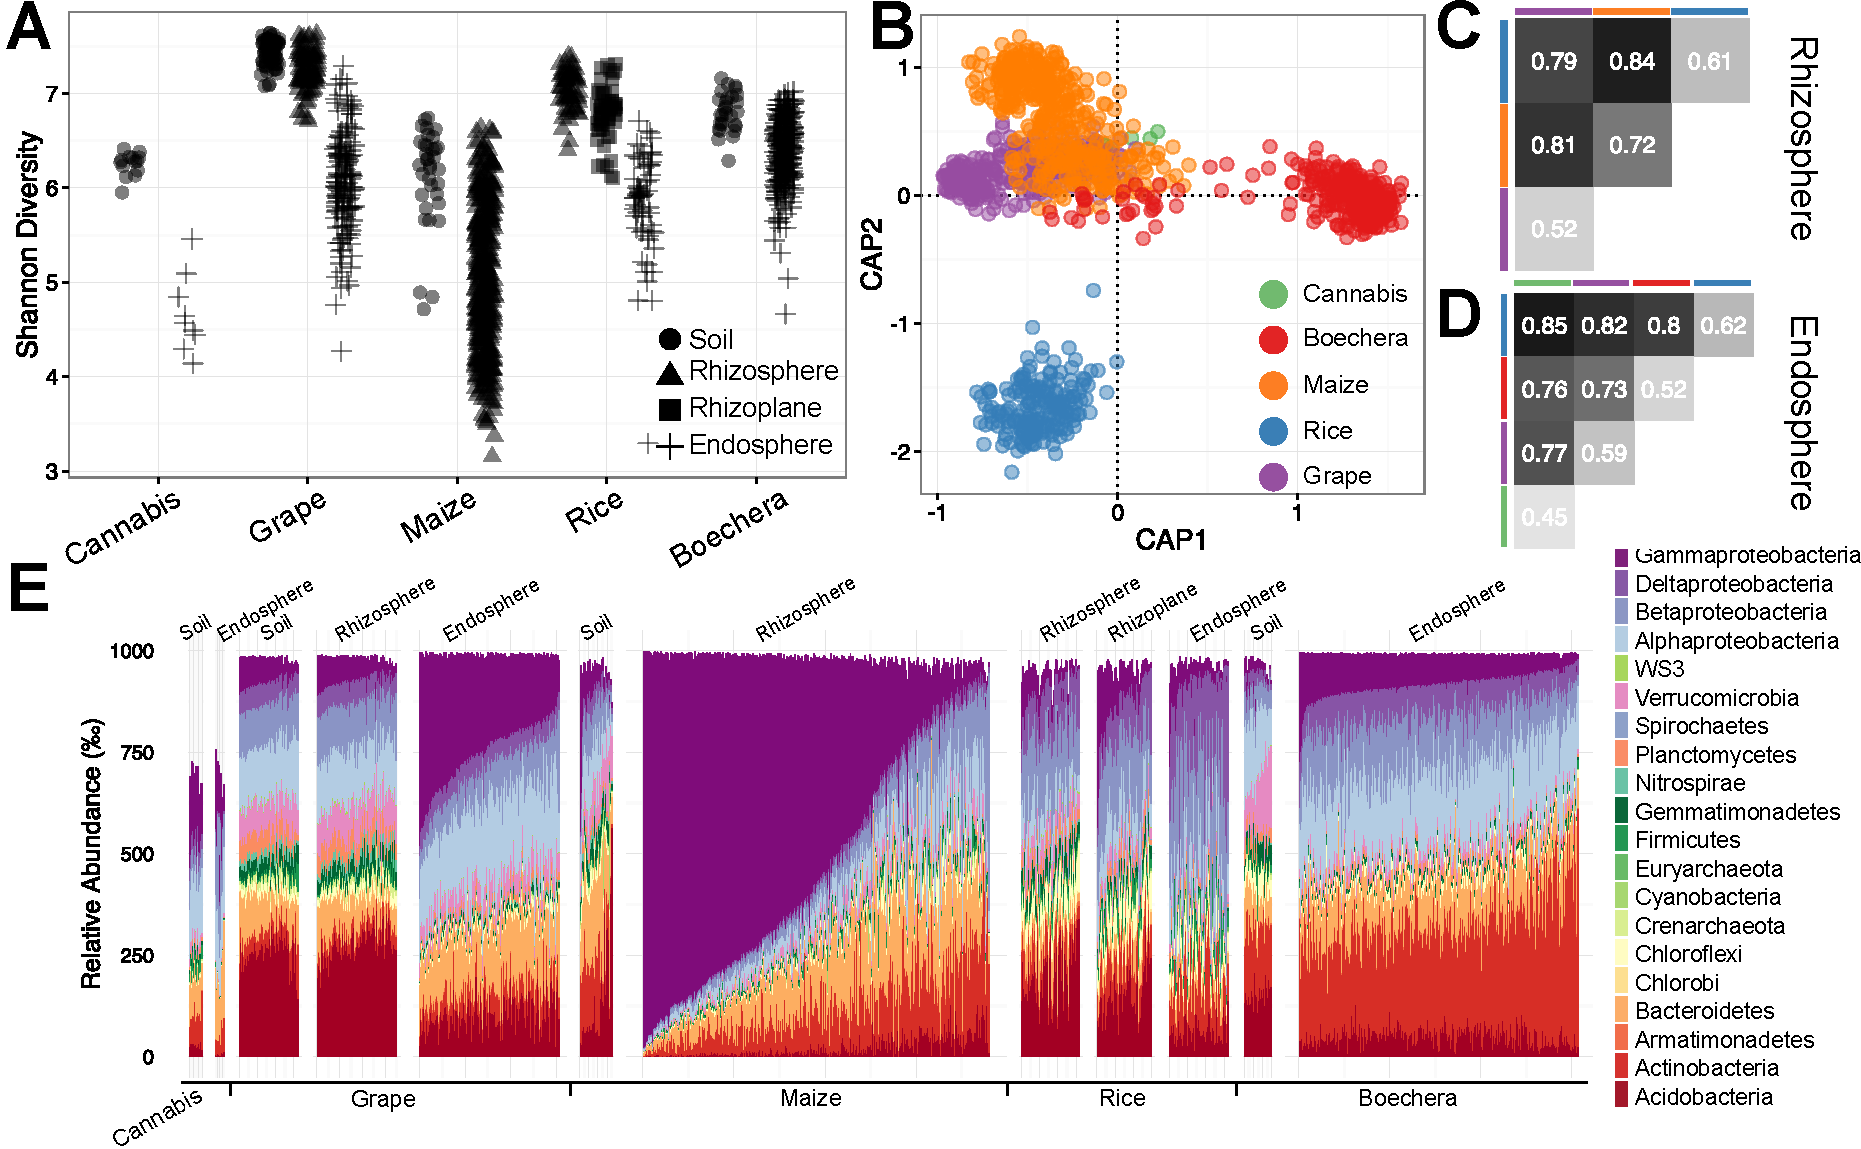
\includegraphics[width=6in]{Figures/figure2_1}
\caption[Figure 3.1]{Figure 1. \textbf{Meta-analysis reveals significant differences among plant rhizospheric microbiomes from different studies.} \textbf{(A)} Shannon diversity estimates of different compartments of plants. \textbf{(B)} CAP analysis using unweighted UniFrac distances. \textbf{(C)} Mean pairwise unweighted UniFrac distances between rhizosphere samples. Colors around boxes represent host species identity and correspond to the color legend in panel B. \textbf{(D)} Mean pairwise unweighted UniFrac distances between endosphere samples. \textbf{(E)} Phylum level abundance between the different compartments of the different plant species.}
\label{fig.sample_1}
\end{figure}

We next used canonical analysis of principal coordinates (CAP) of unweighted UniFrac distances between samples to investigate how interspecies variation affects root associated microbial communities. After constraining the analysis to only focus on the effect of host species on the root-associated microbiomes, we found that root microbial composition varies significantly by host species (R2 = 0.253, P = 0.001), and that their microbiomes cluster distinctly (Fig. 3.1B). We next subsetted the data to analyze the rhizosphere and endosphere compartment separately. Only three of the included studies sampled the rhizosphere compartment. We found that the average unweighted UniFrac distance between rice rhizosphere soil microbiomes and grape rhizosphere soil microbiomes was lower than the rice rhizosphere soil or the grape rhizosphere soil microbiomes compared to the maize rhizosphere (Fig. 3.1C). Additionally the maize rhizosphere microbiome had higher variability than the rice and grape rhizosphere soil microbiomes. For the endosphere fractions, we found that the microbiomes from rice were the most divergent from the other plant species (Fig. 3.1D).

Next, we sought to find which microbial phyla are specifically enriched or depleted in rice compared to the other species (Fig. 3.1E). Because Proteobacteria is the predominant microbial phylum found in the plant root-associated microbiomes, we broke this specific phylum down into its various classes for this analysis. We found that Deltaproteobacteria, Spirochaetes, Firmicutes, Euryarchaeota, Cyanobacteria, Chloroflexi, and Chlorobi were enriched in the rice rhizosphere and endosphere compared to the other plant species, while Armatimonadetes was specifically enriched in the rice rhizosphere soil. We found that Bacteroidetes was depleted in the rice rhizosphere soil and endosphere fractions compared to other plant species, while Alphaproteobacteria and Gammaproteobacteria were specifically depleted in the endosphere of rice compared to the other species.  
Taken together, this data suggests that different plant species acquire significantly distinct root-associated microbiomes and that the rice root endosphere is the most divergent from the other species. While interspecies genetic variation likely has a causal role in the observed variation in the plant root microbiomes, the environment in which plants are grown and technical differences in the studies are also likely to be major drivers of the observed microbiome divergence. For instance, perhaps rice harbors the most divergent microbiome of the included species because it is uniquely growing in submerged soil.


\subsection{Different plant species host distinct microbiotas when growing in the same environment. }
To examine whether rice acquires significantly different root microbial communities than coexisting plant species, we collected roots from rice and various native plant species (Table 3.2) growing in a submerged rice field near Jonesboro, Arkansas (USA). Because plant developmental stage has been implicated in affecting the root microbiota, we collected roots only from plants in the reproductive stage \cite{Lundberg2012}. The bacterial and archaeal communities were analyzed from the rhizosphere soil (soil adhering to the root after shaking, ~1mm from the root surface) and root endosphere compartments. We performed Illumina MiSeq amplicon sequencing of 16S rRNA genes derived from total DNA extracted from the samples and clustered the the amplicon sequences into operational taxonomic units (OTUs) based upon 97\% sequence identity using the NINJA-OPS pipeline \cite{Al-Ghalith2016}.

\begin{table}[ht]
\centering
\small
\definecolor{Gray}{gray}{0.9}
\caption[Table 3.2]{Plant hosts sampled from a rice field.}
\begin{tabular}{c|cc}
\hline
\textbf{Organism}& \textbf{Common Name} & \textbf{Order} \\
\hline
\rowcolor{Gray}
\textit{Oryza sativa}& Asian Rice & Poales \\
\textit{Heteranthera limosa}& Blue Mudplantain & Commelinales \\
\rowcolor{Gray}
\textit{Cyperus flavicomus}& Whiteedge Flatsedge & Poales \\
\textit{Bacopa rotundifolia}& Disk Waterhyssop & Lamiales \\
\hline
\end{tabular}
\end{table}

\begin{figure}[h]
\centering
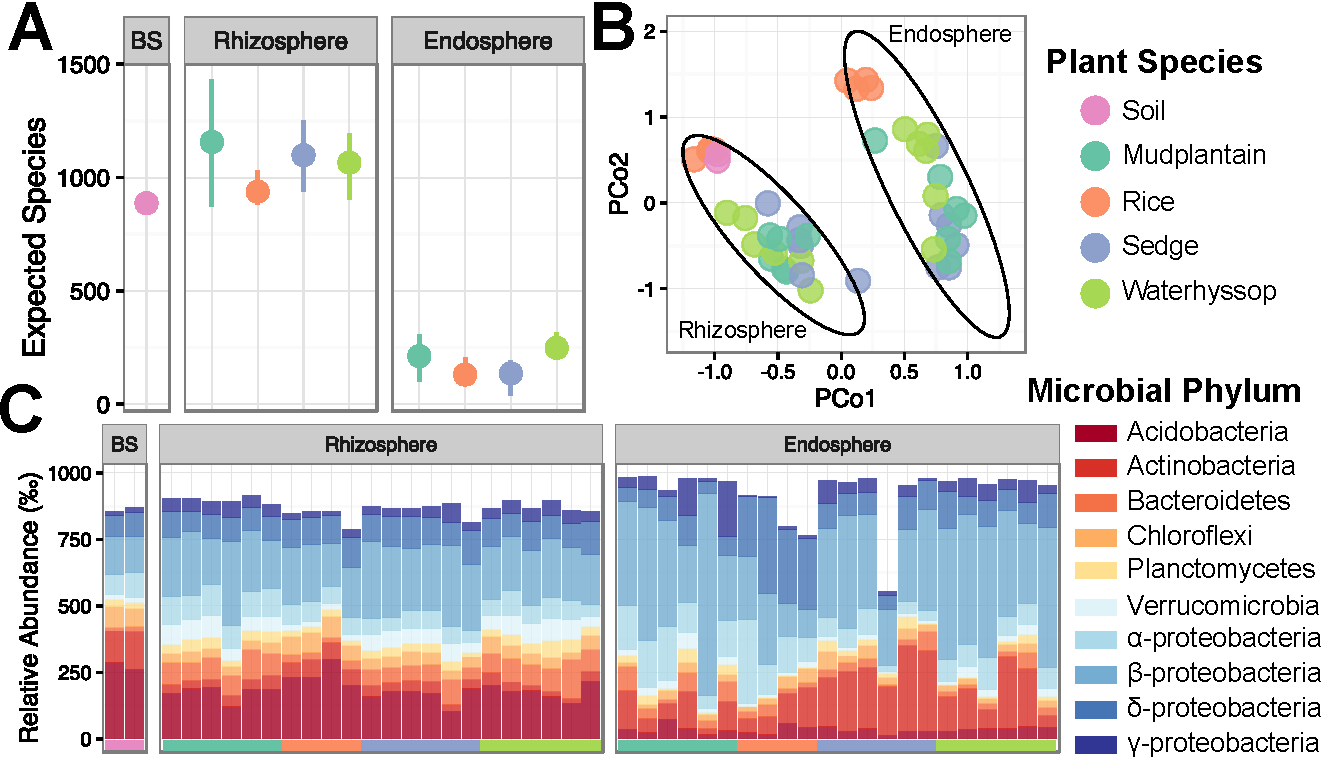
\includegraphics[width=6in]{Figures/figure2_2}
\caption[Figure 3.2]{Figure 2. \textbf{Rice plants and native plants growing in a rice field harbor significantly different rhizospheric microbiomes.} \textbf{(A)} Shannon diversity estimates between compartments and plant species. Points show the mean diversity and tips of bars represent maximum and minimum. The colors of the points match the legend in panel B. BS stands for bulk soil. \textbf{(B)} Principal coordinates analysis using unweighted UniFrac distances. Ellipses mark clustering patterns at 95\% confidence for the rhizosphere and endosphere compartments. \textbf{(C)} Phylum abundances for the different rhizospheric compartments and plant species. Colored bars beneath the x-axis represent the plant species the sample was gathered from and the colors match the legend in panel B.
}
\label{Figure 3.2}
\end{figure}

To inspect the factors governing the patterns of microbial assembly in our dataset, we calculated unweighted UniFrac distances between all samples. After using principal coordinates analysis (PCoA) to visualize clustering patterns of the microbial communities in our samples, we observed that our samples are distinguishable by rhizospheric compartment and by plant species (Fig. 3.2B). We confirmed the statistical significance of these patterns using perMANOVA (Compartment: R2 = 0.23, P < 0.001; Plant Species: R2 = 0.22, P < 0.001). There was a significant interaction term between rhizospheric compartment and plant species (R2 = 0.10, P < 0.001), suggesting that the magnitude of divergence between microbiomes of the different plant species is dependent upon the root compartment. We compared the effect sizes for host species on microbiome composition between each compartment finding that the rhizosphere soil microbiome was more affected by host species (R2 = 0.45, P < 0.001) than the endosphere microbiome (R2 = 0.40, P < 0.001). The differences in microbial community structure were accompanied by divergence in microbial species diversity within samples between compartments (P < 2e-16) and also between plant species (P = 0.026, Fig. 3.2A). We noticed that there were significant differences in species richness between the plant species within the endosphere but not the rhizosphere (P = 0.005 and 0.15, respectively, ANOVA). When comparing the samples collected in this study to the publicly available datasets, we found that native plants collected from a rice field cluster more closely with rice, suggesting that the host plant's environment, i.e. submerged soil, is a more important factor than host plant species in determining the root-associated microbiome (Fig. 3S1).

We noticed significant differences between the different plant species' root microbiotas at the phylum level (Fig. 3.2C). Because root microbiomes are typically dominated by Proteobacterial taxa, we broke the Proteobacteria phylum into its separate classes. Compared to rice, all of the native plants were enriched for Gammaproteobacteria, Bacteroidetes, and Verrucomicrobia in the rhizosphere soil and enriched for Betaproteobacteria and Gammaproteobacteria in the endosphere. Compared to rice, the native plants were depleted for Acidobacteria, Actinobacteria, and Chloroflexi in the rhizosphere soil, and depleted for Deltaproteobacteria in the endosphere. 

\subsection{Rice acquires an outlier microbiome compared to native plant species.}

We compared unweighted UniFrac distances of microbiotas from native plants compared to other native plants and distances of microbiotas from rice plants to native plants. We found that rice root microbiotas are significantly more dissimilar to native plants' microbiotas than native plants' microbiotas are to other native plants (Rhizosphere: P = 4.16e-149, Endosphere: P = 3.58e-148 Fig. 3.3A). This observation could be explained by two scenarios: 1) the native plant species' roots enrich for microbes that are not similarly enriched in rice roots, or 2) rice enriches for a root microbiota that is depleted commonly between the native plant species.

\begin{figure}[h]
\centering
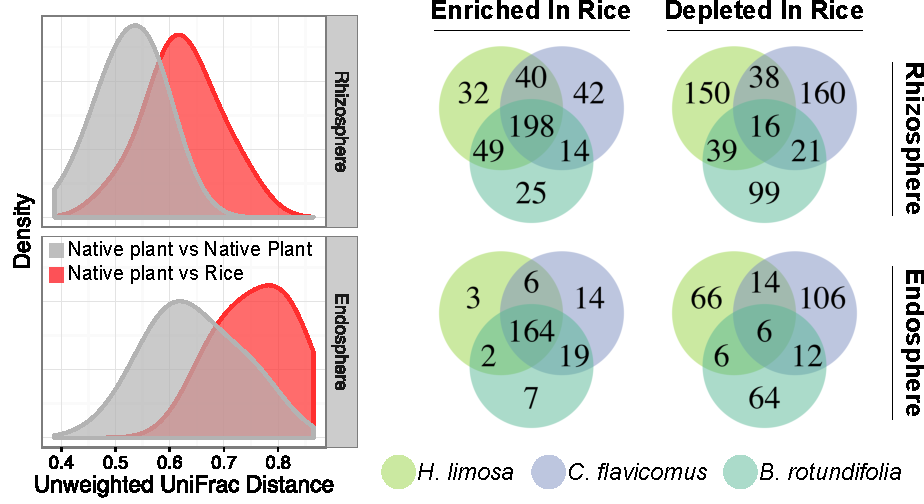
\includegraphics[width=5in]{Figures/figure2_3}
\caption[Figure 3.3]{Figure 3. \textbf{Rice plants acquire an outlier microbiome compared to native plants.} \textbf{(A)} Distribution of unweighted UniFrac distances in each compartment comparing microbiomes from native plants to either rice or other native plants. \textbf{(B)} Results of differential abundance to discover OTUs enriched or depleted in the rice rhizospheric microbiomes compared to native plants.}
\label{Figure 3.3}
\end{figure}

To test these two scenarios, we conducted differential abundance analysis to identify members of the microbiotas that are enriched or depleted in rice compared to the different native plant species. We fit a linear model for each OTU in each rhizospheric compartment to test for differential relative abundance between each native plant species compared to rice. After correcting for multiple testing, we found 1117 unique OTUs that were either significantly enriched or depleted from the rice rhizosphere or endosphere compared to the native plants. When observing the overlap in microbial taxonomies enriched in each native plant species' compared to rice (Fig. 3.3B), we found that 2.4\% of OTUs were in common in the rhizosphere and 1.9\% in the endosphere. Alternatively, of the OTUs depleted in the native plants compared to rice, we found that 22\% of OTUs were in common in the rhizosphere and 28.7\% in the endosphere. Together, these results support the second scenario, where rice enriches for microbes that are consistently depleted from the native plant species. 

\subsection{Rice roots are enriched for methanogenic archaea but not methanotrophic bacteria compared to native plant species.}

Rice cultivation accounts for a large proportion of anthropogenic methane (CH4) emissions. CH4, a powerful greenhouse gas with 80\% greater capacity of trapping heat than carbon dioxide, is produced under anaerobic conditions by certain archaea clades. In a submerged rice field, methanogens derive their energy from degrading rice root exudates and other organic matter derived from decaying straw or roots. While methanogens have been well-characterized in rice field environments, it remains unclear to how specific rice field methanogens are to the rice rhizosphere or whether they may also colonize roots of native plants growing in the same environment.

In the set of differentially abundant microbes we found 8 OTUs belonging to methanogenic taxonomies specifically enriched in the rice rhizosphere and 8 OTUs in the endosphere (with 5 overlapping OTUs). These OTUs belong to the \textit{Methanocella}, \textit{Methanobacterium}, and \textit{Methanosarcina} genera in the rhizosphere and the \textit{Methanobacterium} and \textit{Methanocella} genera in the endosphere. The 8 rice-specific enriched rhizosphere methanogenic OTUs were among the top 10 of 41 most abundant methanogens represented in our rhizosphere dataset, while the 8 of 35 rice root enriched endosphere methanogenic OTUs were among the top 9 most abundant methanogens in our endosphere dataset (Fig. 3.4A). We were unable to identify any methanogenic OTUs enriched in the native plants compared to rice. Indeed, the total relative abundance of methanogenic microbes were enriched in the rice rhizosphere and endosphere compared to native plant species.

\begin{figure}[h]
\centering
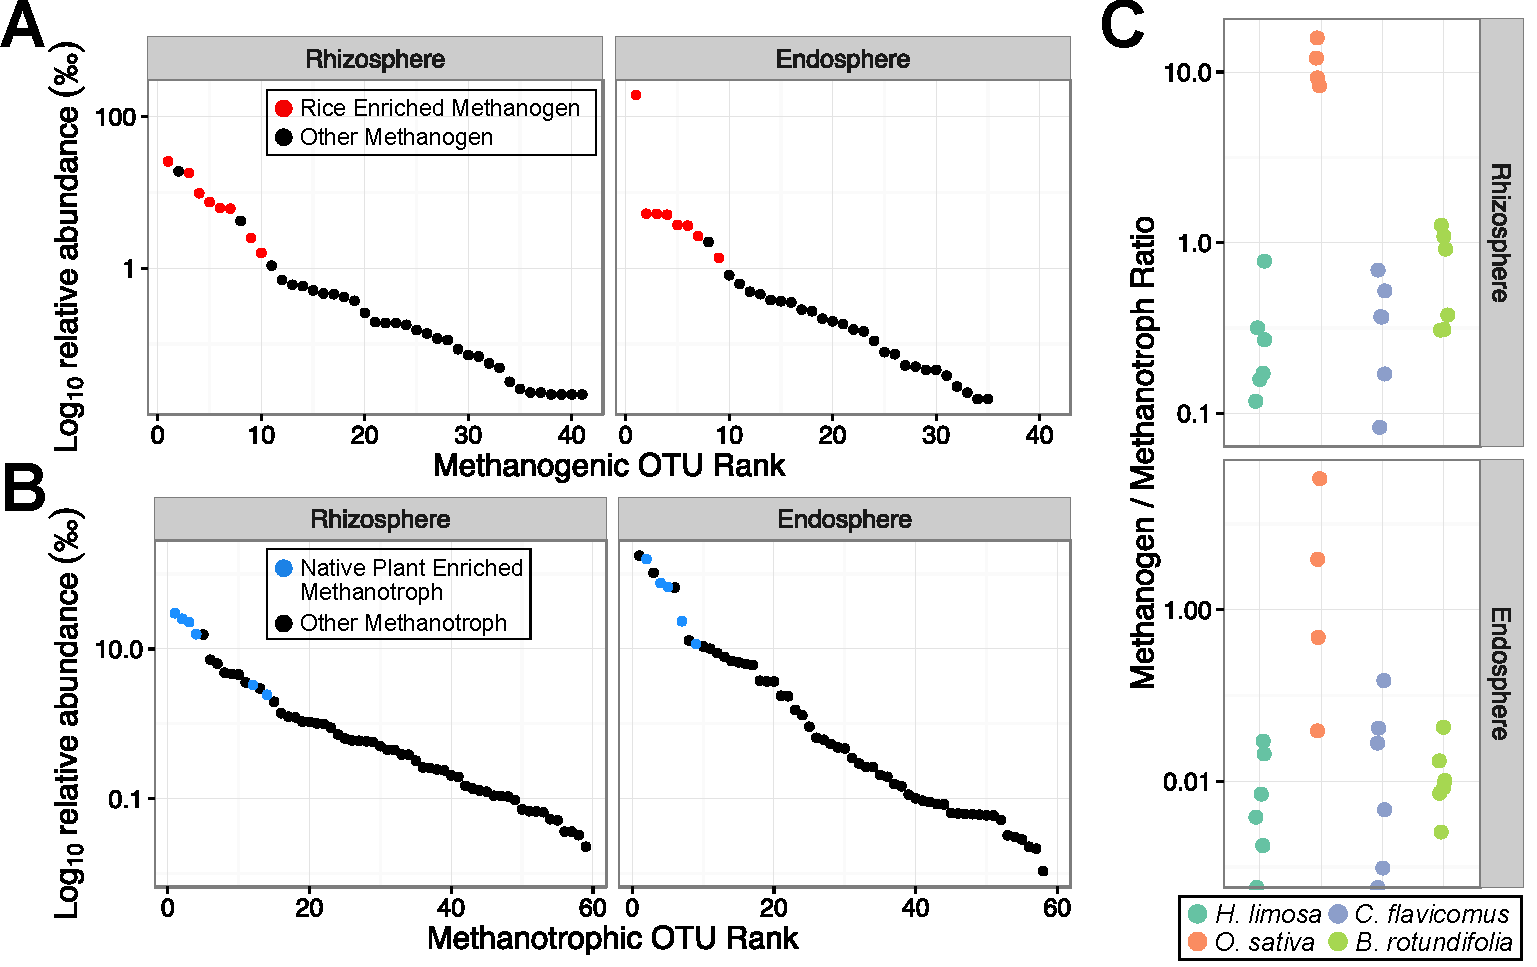
\includegraphics[width=5in]{Figures/figure2_4}
\caption[Figure 3.4]{Figure 4. \textbf{The rice rhizospheric microbiome is enriched for methanogenic microbes.} \textbf{(A)} Rank-abundance plots indicating methanogens enriched in the rice rhizosphere soil and endosphere microbiomes. \textbf{(B)} Rank-abundance plots indicating methanotrophic eubacteria enriched in the native plant microbiome. \textbf{(C)} Methanogen to methanotroph ratios in each compartment of each plant species.}
\label{Figure 3.4}
\end{figure}

Methane can be oxidized by methanotrophic eubacteria under aerobic conditions. Methanotrophs have previously been reported to inhabit the rice rhizosphere soil, rhizoplane, and endosphere and thus may partially mitigate CH4 release into the atmosphere. We were interested in how methanotrophic populations differ between host species' rhizospheres and whether different plant species enrich for certain methanotrophic taxa. In rice, we found two OTUs to be significantly enriched in the endosphere compared to at least one native plant species (with one OTU 4752 being enriched compared to \textit{C. flavicomus} and OTU 4736 being enriched compared to \textit{B. rotundifolia}). Both of these OTUs belong to the Methylosinus genus. These two OTUs, however, were not significantly enriched in the rice endosphere compared to the other native plants, suggesting that OTU 4752 and OTU 4736 are specifically depleted in the \textit{C. flavicomus} and \textit{B. rotundifolia} endospheres, respectively. 

We next looked for methanotrophs that were significantly enriched in the rhizosphere or the endosphere of at least one native plant compared to rice. We found 6 unique methanotrophic OTUs enriched in the rhizosphere and 5 unique methanotrophic OTUs enriched in the endosphere of at least one native plant compared to rice. The rhizosphere enriched methanotrophs were among the top 14 of 59 most abundant methanotrophs in our rhizosphere dataset and the endosphere enriched methanotrophs were among the top 9 of 58 most abundant methanotrophs in our endosphere dataset (Fig 3.4B). Overall relative abundance of methanotrophs was significantly higher in the rhizosphere of native plants than rice (P = 4.789e-09, Welch two sample t-test), but not the endosphere (P = 0.749, Welch two sample t-test).

We next compared the relative abundance ratios of methanogenic archaea to methanotrophic bacteria in each plant species. The rhizosphere generally had higher ratios of methanogens to methanotrophs compared to the endosphere (Fig. 3.4C). This is expected as roots contain the highest levels of oxygen in an otherwise anoxic environment and methanotrophs flourish under aerobic conditions (while the opposite is true for methanogens). We found that rice has a significantly higher ratio of methanogenic microbes than methanotrophic bacteria in both the rhizosphere and endosphere compared to native plants growing in the same environment. The native plants had mean ratios < 1 in both the rhizosphere and endosphere, while rice had mean ratios > 1 in both the rhizosphere and endosphere. Without knowing the activity levels of the methanogens and methanotrophs in our dataset it is impossible to definitively declare whether the rice root microbiome is a net producer of CH4 and the native plants' microbiomes are net CH4 sinks, however it is reasonable to assume that the rice root microbiome produces more CH4 than the native plants'. 

\subsection{Soil cultivation history affects plant root microbial assemblages.}
When comparing the rhizosphere soil microbial community structure to that of unplanted (bulk) soil from the same field site, we noticed that rice rhizosphere soil communities are significantly more similar to bulk soil microbial communities than are native plant rhizosphere soil communities (Fig. 3.2B and Fig. 3.5A). Endosphere microbial community structure of the tested plant species, however, differed equidistantly from bulk soil communities. Two non-mutually exclusive hypotheses arise from these results. The first hypothesis is that dense monoculture of rice over the course of multiple years can change the soil's microbiome to be more similar to that of the rice rhizosphere. Many rice fields in the USA are planted densely such that nearly all areas within a field are impacted by rice roots, thus most of the surface soil is rhizosphere. The second hypothesis is that, compared to the native plants growing in the field, rice has a weaker ability of differentiating its rhizosphere microbiome from that of the surrounding soil microbial communities. 

\begin{figure}[h]
\centering
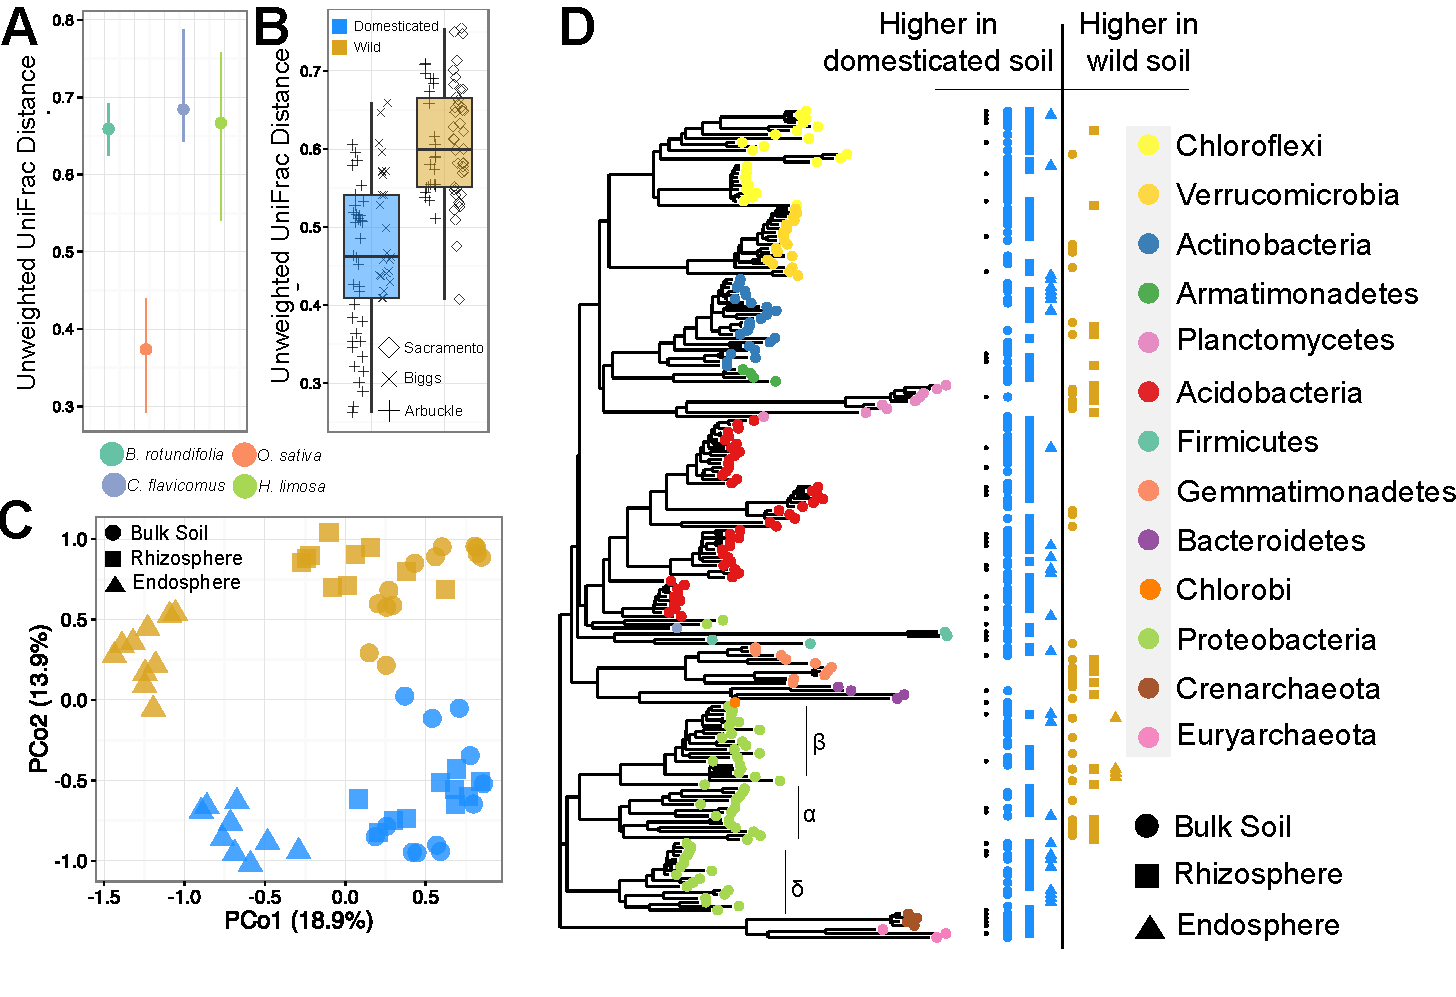
\includegraphics[width=6in]{Figures/figure2_5}
\caption[Figure 3.5]{Figure 5. \textbf{Rice cultivation has an impact on the overall soil microbiome.} \textbf{(A)} Unweighted UniFrac distances between the rhizosphere soil microbiomes of rice and native plants compared to unplanted soil from the same field. \textbf{(B)} Unweighted UniFrac distances between the microbiomes of unplanted wild or domesticated soils from different locations and the assembled rhizosphere soil microbiomes of isogenic rice grown in each soil. \textbf{(C)} Principal coordinates analysis of unweighted UniFrac distances of microbiomes sampled from isogenic rice plants growing in domesticated and wild soil from different sites. \textbf{(D)} Phylogenetic tree showing relationship between OTUs found to be enriched in microbiomes from wild and domesticated soils. Black points represent OTUs found to be specifically enriched in rice compared to native plants (Fig. 3.3B).}
\label{Figure 3.5}
\end{figure}

To test the first hypothesis, we grew rice plants (cultivar M206) in soil from two rice fields (from here on referred to as domesticated soil) as well as soil from two non-agricultural sites (i.e. soils in which no crop plants have been grown, from here on referred to as wild soil) under controlled conditions. This experiment was carried out in two batches. In the first batch, plants were grown in a domesticated soil from Arbuckle, CA and a wild soil from Sacramento, CA. In the second batch, rice plants were grown in a domesticated soil from Biggs, CA and a wild soil from Arbuckle, CA. Along with unplanted soil controls, we collected DNA from rhizosphere and endosphere samples and sequenced the V4 region of the 16S rRNA gene. The root microbial communities acquired from wild soils were significantly different and clustered distinctly from microbiomes those acquired from domesticated soil (Fig 5C, R2 = 11.9, P = 0.001). We noticed a significant interaction term between soil history and root compartment (R2 = 0.063, P = 0.001, PerMANOVA). Although each compartment's microbiome was significantly affected by soil history, the rhizosphere communities were more affected by soil history than the endosphere communities (R2 = 0.30 vs 0.22, respectively, P = 0.001, PerMANOVA). The rhizosphere soil microbiota of plants growing in wild soils were significantly more distant to unplanted soil controls than rhizosphere soil microbiotas of plants growing in domesticated soils (Fig. 3.5B, P = 7.29e-16, ANOVA). Root-associated microbiomes assembled from wild soil had greater variability than those assembled from domesticated soils (Fig. 3S2 Rhizosphere: P = 0.006, Endosphere: P = 0.019). Taken together, these observations support the hypothesis that rice cultivation “domesticates” the microbiome of the soil environment to be more similar to the rice rhizosphere microbiome.

We were next interested in finding individual taxa responsible for the acquired microbiome differences between plants grown in domesticated and wild soil. Again we used a linear model approach where the log2 abundance of each OTU in each rhizospheric compartment was modeled as a function of soil history status. Because this experiment was carried out in two batches, we decided to model each experimental batch separately and find the overlap of OTUs that were significantly enriched in each compartment of domesticated and wild soils between the batches. We found a total of 252 OTUs to be enriched in the bulk soil, rhizosphere, and endosphere of domesticated soil (165 unique OTUs) while we found 60 OTUs to be enriched in the bulk soil, rhizosphere, and endosphere of plants grown in wild soil (47 unique OTUs). Soil cultivation history appeared to broadly affect the abundance of individual taxa from several phyla: Acidobacteria, Verrucomicrobia, Chloroflexi, Euryarchaeota, and Actinobacteria members were enriched in the bulk soil, rhizosphere, or endosphere of plants grown in domesticated soils, while Gemmatimonadetes and Planctomycetes members were more present in the microbiomes assembled from wild soils (Fig. 3.5D, hypergeometric test, adjusted P <= 0.05). Similarly, we found that members of the Deltaproteobacteria class are uniquely enriched in the domesticated soil assemblages. 

We compared the OTUs that were found to be significantly enriched in the microbiomes assimilated from domesticated soils to those OTUs found to be specifically enriched in the rice rhizosphere and endosphere microbiomes compared to native plants. Of the 165 unique OTUs enriched in microbiomes originating from the domesticated soils, we found an overlap of 46 OTUs between the rice specific taxa (black data points, Fig. 3.5D). The magnitude of this overlap was greater than expected by chance alone (P = 0.0008, hypergeometric test), implying that rice plant physiology is a major structuring factor for rice field soil microbiomes.

\section{Discussion}
Our analysis of various plant species cultivated in different environments demonstrates that rice assembles a relatively distinct root-associated microbiome amongst crop species, likely because of the submerged conditions under which the plants are cultivated (Fig. 3.1B). Indeed, after sampling the roots of native plants growing in a rice field, we observed that soil submergence has a clear effect on root-assembled microbiomes (Fig. 3S1). However, we found that despite growing under submerged conditions, root-associated microbiomes are significantly dependent upon plant species. The three native plants species, each of which is a common weed found in rice fields across the U.S., assemble microbiomes with profiles clustering distinctly from rice. Through differential abundance analysis, we determined that the rice microbiome clusters separately from the native plant species' microbiomes due to rice roots enriching for a relatively unique microbiome. Conversely, the taxa enriched in the native plant microbiomes (compared to rice) overlap to a much reduced extent. We found that root-associated microbiome differences species were disjunct from host plant phylogeny. Similar results were reported in Arabidopsis relatives \cite{Schlaeppi2014}. In a study comparing domesticated rice species to wild rice species, it was found that microbiome differences only weakly correlated with phylogenetic differences; however, larger microbiome differences were observed based upon domestication status \cite{Shenton2016}. Together, these results suggest that the culmination of physiological traits governing root-associated microbiome assembly may be arrived at through convergent evolution. 

Methane emission from rice paddies is a complex phenomenon governed by many environmental factors \cite{Minami1994}. We found that the rice root-associated microbiome is enriched for methanogenic archaea compared to the native plants. Rice plants host a higher methanogen to methanotroph ratio than the native plants, suggesting that methane emission levels from submerged environments may be host species-specific. Early divergent members of the \textit{Oryza} genus were also found to host a higher proportion of methanotrophic eubacteria \cite{Shenton2016}. Taken together, these results indicated that domestication of rice may have indirectly selected for a microbiota with a higher capacity for hosting methane producing microbes. The root architectural and physiological parameters governing methanogen to methanotroph ratios in root microbiomes remain elusive; however, native plant species growing in similar environments as rice may be a resource for understanding the physiological and root architectural parameters governing associations between plants and methanogens and methanotrophs. Because CH4 emissions vary significantly across rice genotypes \cite{Simmonds2015}, CH4 emission could be treated as a complex trait and correlated with genomic loci to have a better mechanistic understanding of which plant traits govern the composition of rhizospheric microbiomes in respect to greenhouse gas emissions.

Intensive agriculture has unknown consequences on the microbiota of agricultural ecosystems. We observed that the rice rhizosphere soil microbiome is significantly less dissimilar to unplanted soil communities than are those of native plants. We proposed two non-mutually exclusive hypotheses for this: 1) intensive cultivation over multiple seasons allows the roots of rice plants to modify the soil microbiome to be more like the rice rhizosphere and 2) that rice has a weaker ability to differentiate its rhizosphere soil microbiome from the surrounding soil microbiome than native plants. While we were unable to address the latter hypothesis in this study, we tested the first hypothesis by growing rice plants in soils collected from non-agricultural locations (i.e. wild soils, soils from uncultivated land) and soils from rice fields (i.e. domesticated soil). In support of our hypothesis, we found that the rhizospheric soil microbiomes assembled from wild soils were more dissimilar to their corresponding bulk soils than were plants grown in domesticated soils. Furthermore, we found that soil history has a prominent effect on both the rhizosphere soil and endosphere microbiomes. Community structure variability was significantly higher within the rhizosphere and endosphere microbiomes assembled from wild soils compared to the domesticated soils, suggesting that rice cultivation selects for a consistent microbiome. While our results support the hypothesis that rice plants exert a large effect on the soil microbial communities in rice fields, we cannot exclude the possibility that native plants also have a stronger ability to differentiate their rhizospheric microbiomes from that of the surrounding soil. 

Despite variability in wild soils, we found that assembled microbiomes are discernible based upon soil history. These differences are reflected in the taxa that have significantly different relative abundances between the microbiomes assembled from the two soil types. We found many more taxa to be enriched in the microbiomes assembled from domesticated soils than from wild soils, consistent with the observation of higher community variability in wild soils. We observed a significant overlap of 65 OTUs between domesticated soil enriched OTUs and rice specific enriched OTUs from the native plant study. This statistic is impressive given that the studies were conducted in two disparate, but rice cultivating, regions of the United States. Taken together, these results imply that agricultural soil microbiomes are not only shaped by cultivation practices \cite{Edwards2015}, but also by unique aspects of the crop plants' physiologies. The functional benefits and / or disadvantages of modifying soil microbiomes to better resemble a plant's rhizospheric microbiome are unknown. Amending soil quality and nutrition by rotating cover crops in agricultural settings has been employed by farmers for centuries but, the functional link between soil health and microbial community structure remains largely unresolved. Understanding the relationship between crop physiology, rotation, and productivity and plant-microbe and microbe-microbe interactions should thus be an important focus of future research.

\section{Materials and Methods}
\subsection{Meta-Analysis}
Assembled 16S rRNA gene sequences and metadata were downloaded from the QIITA database for maize (Peiffer et al. 2013, QIITA ID number: 1792), grape (Zarraonaindia, et al., QIITA ID number: 2382), and cannabis (Winston et al., 2013, QIITA ID number: 1001). Sequences for Boechera (Wagner et al. 2016) were downloaded from European Nucleotide Archive (study number: PRJEB10570) and metadata was downloaded from the study's associated Dryad repository (http://datadryad.org/resource/doi:10.5061/dryad.g60r3). The paired-end sequences were trimmed to remove primer regions and then assembled into contiguous sequences using PANDAseq \cite{Masella2012}. For the rice dataset, we only used sequences from field grown plants in Edwards et al. 2015 \cite{Edwards2015}. Assembled reads were discarded if containing any ambiguous bases or if the read was less than 275 bases in length. The sequences were clustered based upon 97\% sequence identity into operational taxonomic units (OTUs) against the GreenGenes \cite{DeSantis2006} 13\_8 database using the NINJA-OPS pipeline \cite{Al-Ghalith2016}. NINJA-OPS is a closed-reference, fast, and memory efficient pipeline that uses bowtie2 \cite{Langmead2012} to map amplicon reads to a simulated chromosome (concatenated reference sequences from the GreenGenes 13\_8 database).

\subsection{Native Plant Study}
Roots with attached soil from rice and native plants, along with unplanted soil, were collected from a single rice paddy near Jonesboro, Arkansas (USA) on August 22, 2015. Rhizosphere and endosphere fractions from each host plant was collected according to the methodology used previously \cite{Edwards2015}. The roots were shaken by hand to remove loosely bound soil and then placed into 50 mL Falcon tubes with 15 mL of sterile PBS solution. The samples were stored on ice and shipped overnight to the University of California, Davis. Upon receiving the samples, the rhizosphere soil fraction was removed from the roots by vortexing in PBS solution and 500 $\mu$L of the resulting soil slurry was placed into a sample tube for DNA extraction. The roots were vortexed in consecutive washes of fresh PBS solution until all soil was depleted and then sonicated 3 times at (x Hz) for 30 seconds in fresh PBS to remove all rhizoplane microorganisms. The remaining roots were placed into a sample tubes for DNA extraction. All DNA extractions were performed using the MoBio Powersoil DNA isolation kit. 

\subsection{Soil Domestication Study}
The soil domestication study was conducted in two batches using 4 different soils. In the first batch, soil was collected on April 10, 2015 from a non-agricultural site near Sacramento, California and from a rice field near Arbuckle, California. The second batch of soils was collected on June 3, 2016 from a non-agricultural site near Arbuckle, California and a rice field at the Rice Experiment Station in Biggs, California. The soils were brought back to the greenhouse, homogenized, placed into pots, and inundated with water. Axenic rice seedlings (see method below) were transplanted into each pot and supplemented with nutrient solution every 14 days. For each batch, roots were harvested from the plants 6 weeks after transplantation. The roots were shaken to remove loosely attached soil, leaving ~1mm of soil attached. Compartment separation and DNA isolation was performed as described above.

\subsection{Seed Sterilization and Germination }
Rice seeds were stripped of their hulls by vigorous back and forth rolling in a 5 inch cut portion of a bicycle tire tube. The seeds were shaken in 70\% bleach for 5 minutes then washed three times in autoclaved deionized water. Using ethanol flamed forceps, the seeds were then transferred into petri plates containing half strength MS agar (1\%). The plates were placed in a dark growth chamber at $30\,^{\circ}\mathrm{C}$ for 7 days. The seeds were then placed upon the bench top in order to de-etiolate. Any plates containing fungal or bacterial growth were discarded.

\subsection{16S rRNA gene amplification and sequencing} 
All 16S rRNA gene amplification was performed as noted in Edwards et al., 2015. Briefly, the V4 region of the 16S rRNA gene was amplified using PCR with a dual indexing strategy. For each PCR reaction, a corresponding negative control was also performed. All reactions were checked for amplification by running PCR products out on a 1\% agarose gel. If a reaction's negative control succeeded in amplification, then we discarded the particular reaction and reperformed the PCR. The PCR reactions were purified using AMPure beads and measured for concentration using a Qubit. The PCR products were pooled in equimolar concentrations, concentrated using AMPure beads, and then gel extracted from a 2\% agarose gel. Sequence libraries were sent to the University of California DNA Technologies Core Laboratory for 250 x 250 bp sequencing on the Illumina Miseq platform. 

\subsection{Sequence processing}
The resulting paired end sequences were demultiplexed using custom Python scripts and aligned into contiguous reads using PANDAseq \cite{Masella2012}. The contiguous reads were discarded if containing any ambiguous bases or if the length exceeded 275 bases. All reads were then clustered into OTUs based upon 97\% sequence identity using NINJA-OPS as described above. OTUs with plastid and mitochondrial taxonomies were removed from all resulting OTU tables. All scripts used for sequence processing can be found at (github).

Statistical Analysis Weighted and Unweighted UniFrac distances were calculated using QIIME \cite{Caporaso2010}. All other statistical analyses were conducted using R version 3.1 \cite{RCoreTeam2016}. Unless otherwise noted, we determined statistical significance at $\alpha$ = 0.05 and, where appropriate, corrected for multiple hypothesis testing using the Benjamini and Hochberg method \cite{Benjamini1995}. Shannon diversity was calculated using the diversity() function, PCoA and CAP analyses were conducted using the capscale() function, perMANOVA was conducted using the adonis() function, and community structure variability was measured using the betadisper() function all from the Vegan package \cite{Oksanen2013}. Linear models were run using the lm() function and ANOVA was run using the aov() function. Hypergeometric tests were run using the phyper() function. Phylogenetic trees were displayed using the plot\_tree() command from the PhyloSeq package \cite{McMurdie2013}. All other graphs and plots were generated using the ggplot2 package \cite{Wickham2009}. R notebooks for the full analyses can be found (github).

\newpage

\begin{figure}[h]
\centering
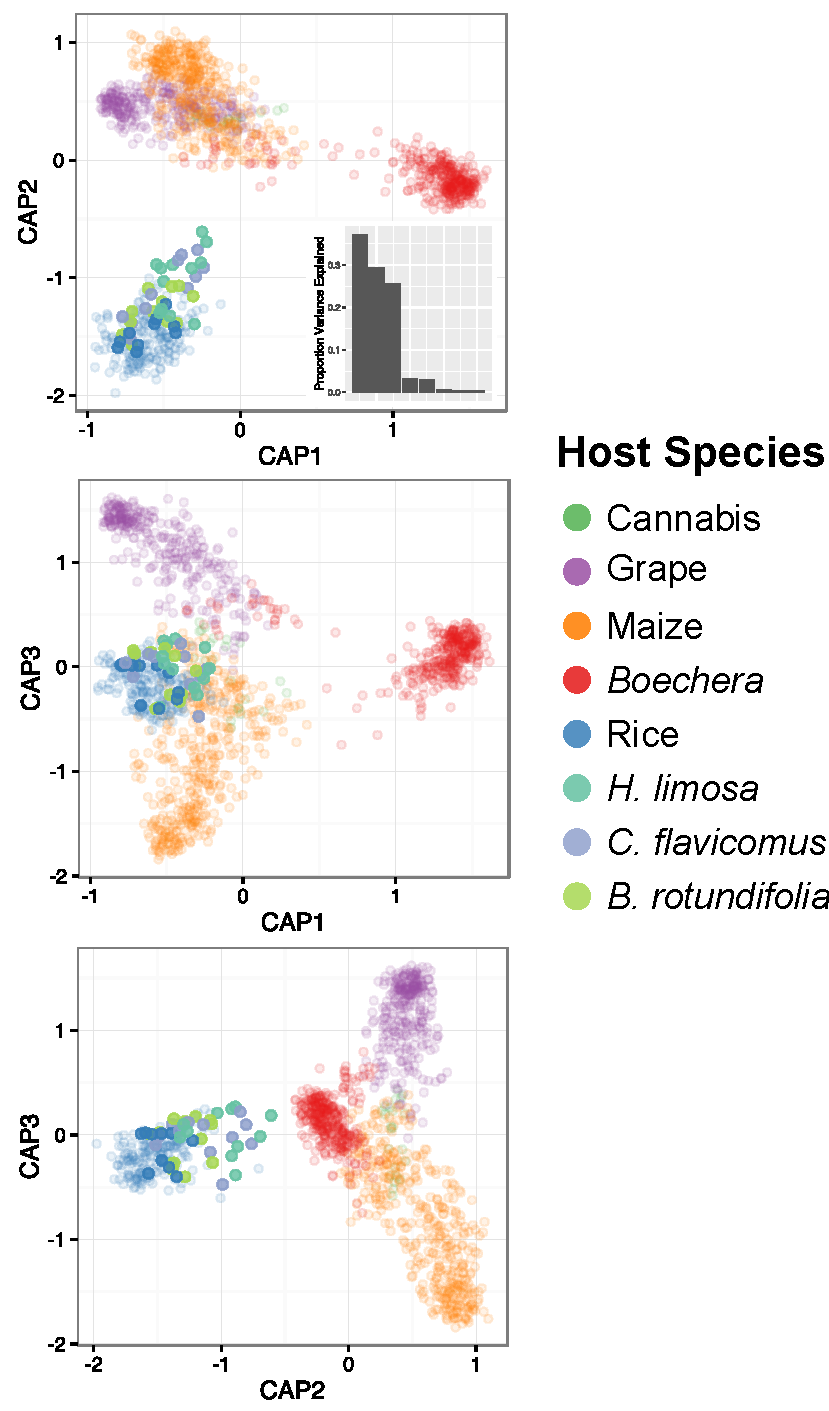
\includegraphics[width=4in]{Figures/figure2_s1}
\captionsetup{labelformat=empty}
\caption[Figure 3S1]{\textbf{Figure 3S1. CAP analyses of published datasets displaying where the native plants taken from an Arkansas rice field cluster along the first three axes.} The inset in the uppermost panel depicts the amount of variance explained by each axis.}
\label{Figure 3S1}
\end{figure}

\newpage

\begin{figure}[h]
\centering
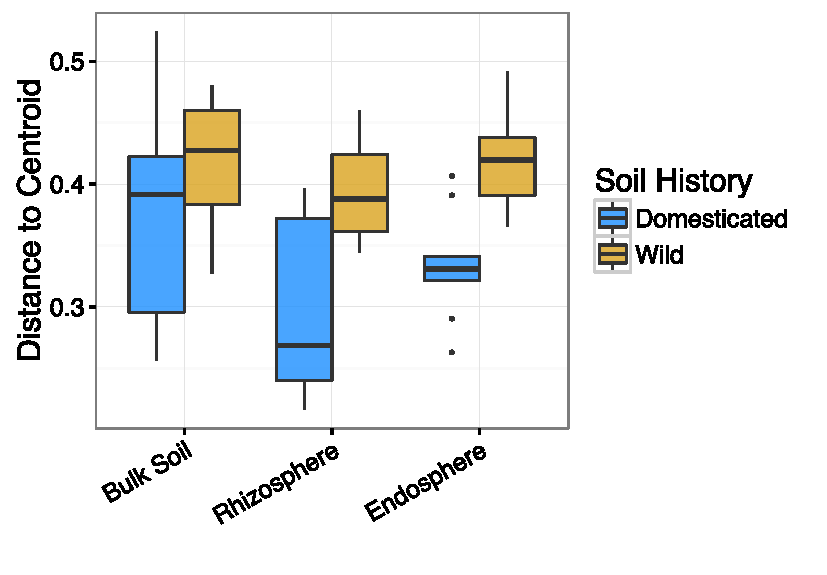
\includegraphics[width=4in]{Figures/figure2_s2}
\captionsetup{labelformat=empty}
\caption[Figure 3S2]{\textbf{Figure 3S2. Dispersion of beta diversities for each sample type from domesticated and wild soils.}}
\label{Figure 3S2}
\end{figure}